\documentclass{article}
\usepackage[utf8]{inputenc}
\usepackage{geometry}
\geometry{
  a4paper,
  total={170mm,257mm},
  left=20mm,
  top=20mm,
}
\usepackage{graphicx}
\usepackage{titling}
\usepackage{booktabs}
\usepackage{listings}
\usepackage{xcolor}
\usepackage{hyperref}
\usepackage{fancyvrb}
\usepackage{float}
\usepackage{amsmath}

\definecolor{darkblue}{rgb}{0.0, 0.0, 0.5}
\RecustomVerbatimEnvironment{verbatim}{Verbatim}{formatcom=\color{darkblue}}
\setlength{\parindent}{0pt}

\title{\textbf{DEEP LEARNING} \\
{\Large \textbf{Report 2: Linear Regression}}}
\date{May 2026}

\usepackage{fancyhdr}
\fancypagestyle{plain}{
  \fancyhf{}
  \fancyfoot[L]{\thedate}
  \fancyfoot[R]{\thepage}
  \fancyhead[L]{University of Science and Technology of Hanoi}
  \fancyhead[R]{Deep Learning}
}
\makeatletter
\def\@maketitle{%
  \newpage
  \vskip 1em
  \begin{center}
  \let \footnote \thanks
    {\LARGE \@title \par}%
    \vskip 1em
  \end{center}
  \par
  \vskip 1em}
\makeatother

\begin{document}
\pagestyle{plain}
\maketitle

\noindent\begin{tabular}{@{}ll}
  Student: & Vu Ha Vy -- 2540112 \\
\end{tabular}

\section*{Implementation}

\subsection*{Loss Function}

The loss function measures how far the model's predictions are from the true
values. For each data point, the model predicts $\hat{y}_i = w_1 x_i + w_0$.
The overall loss is the Mean Squared Error averaged over all $N$ points:
\[
  J(w_0, w_1) = \frac{1}{2N} \sum_{i=1}^{N} (\hat{y}_i - y_i)^2
\]


\begin{verbatim}
def loss(data, w0, w1):
    N = len(data)
    Z = 0.0
    for xi, yi in data:
        y = w1 * xi + w0
        Z += (y - yi) ** 2
    return 0.5 * Z / N
\end{verbatim}

\subsection*{Gradient Descent}

To minimize $J$, we compute the partial derivatives of $J$ with respect to
each parameter and move the weights in the opposite direction of the gradient:
\[
  \frac{\partial J}{\partial w_0} = \frac{1}{N}\sum_{i=1}^{N}(w_1 x_i + w_0 - y_i)
  \qquad
  \frac{\partial J}{\partial w_1} = \frac{1}{N}\sum_{i=1}^{N} x_i \cdot (w_1 x_i + w_0 - y_i)
\]

\begin{verbatim}
def gradient_descent(data, lr, thres):
    w0 = 0.0
    w1 = 1.0

    N = len(data)
    i = 0
    J_prev = float('inf')

    while True:
        i += 1

        J = loss(data, w0, w1)

        if abs(J - J_prev) < thres:
            print(f"Converged at iteration {i}, J = {J}")
            break

        J_prev = J

        print(f"{i} | {w0:.4f} | {w1:.4f} | {J:.4f}")

        dw0 = 0.0
        dw1 = 0.0

        for xi, yi in data:
            z = w1 * xi + w0 - yi
            dw0 += z
            dw1 += xi * z

        dw0 /= N
        dw1 /= N

        w0 = w0 - lr * dw0
        w1 = w1 - lr * dw1

    return w0, w1
\end{verbatim}

\section*{Dataset}

The dataset \texttt{lr.csv} contains 5 data points:

\begin{table}[H]
\centering
\begin{tabular}{cc}
\toprule
$x$ & $y$ \\
\midrule
10 & 55  \\
20 & 80  \\
40 & 100 \\
60 & 120 \\
80 & 150 \\
\bottomrule
\end{tabular}
\caption{Contents of \texttt{lr.csv}}
\end{table}

\section*{Results}

With learning rate $r = 0.0001$ and threshold $t = 10^{-6}$, the algorithm
converged after \textbf{179622 iterations} with final loss $J = 9.4697$.
The learned model is:
\[
  \hat{y} = 1.2686 \cdot x + 47.6189
\]

\begin{figure}[h]
    \centering
    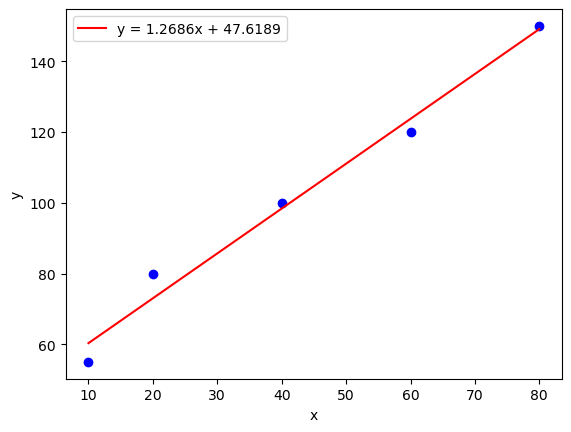
\includegraphics[width=0.6\textwidth]{plot.png}
\end{figure}

\subsection*{Effect of Learning Rate}

The learning rate $r$ controls how large each update step is.
Table below compares three values of $r$ with the same threshold
$t = 10^{-6}$.

\begin{table}[H]
\centering
\begin{tabular}{ccccc}
\toprule
Learning rate $r$ & Iterations & Final loss $J$ & $w_1$ & $w_0$ \\
\midrule
$0.00001$ & 1371377 & 9.6357 & 1.2624 & 46.8211 \\
$0.0001$  & 179622             & 9.4697 & 1.2686 & 47.6189 \\
$0.0005$  & 41863              & 9.4549 & 1.2651 & 47.8228 \\
\bottomrule
\end{tabular}
\caption{Comparison of learning rates (threshold $t = 10^{-6}$)}
\label{tab:lr}
\end{table}

A larger learning rate converges much faster, $r = 0.0005$ needed only
41,863 iterations compared to over 1.3 million for $r = 0.00001$.
All three runs produce very similar models, with $w_1 \approx 1.26$ and
$w_0 \approx 47$, so the choice of $r$ does not affect the final result,
only the speed. Setting $r$ too large (e.g.\ $r = 0.01$) will cause the
weights to overshoot.

\end{document}